\chapter{Algorithmic Efficiency on Modern CPU Architectures}
\label{chap:efficienza-cpu}

\FloatBarrier
\section{The Role of Efficiency in Information Retrieval}

The development of information processing systems unfolds along two complementary dimensions that are often in tension with one another:

\begin{enumerate}
    \item \textbf{Effectiveness:} maximizes end-user satisfaction, focusing on the semantic quality of results, ranking, and natural language processing, typically using high-level abstraction tools (Python, Machine Learning frameworks).
    \item \textbf{Efficiency:} minimizes infrastructural operating costs, designing algorithms optimized down to the last CPU clock cycle and the last bit of occupied memory.
\end{enumerate}

No single professional figure is required to master both extremes; however, those who develop at a high level must understand the physical constraints of the underlying hardware to avoid designing impractical solutions, while those who optimize at a low level must preserve the structure and semantics of the data so as not to compromise its effectiveness.

\subsection{The Three Pillars of Efficiency in IR Systems}

\paragraph{User experience.} In web-scale systems, a query response must be delivered within an infinitesimal fraction of a second. Users perceive any delay beyond a few tenths of a second: if results are slow or irrelevant, they abandon the service in favor of a competitor. Algorithmic efficiency does not only serve to respond faster, but allows more sophisticated and effective ranking and filtering algorithms to run \emph{within the same predetermined time budget} (typically a hard ceiling of $100$--$200\,\text{ms}$).

\paragraph{Operational scalability.} Modern systems handle billions of documents, multimedia items, queries, and logs generated every second. The number of machines required is approximately:
\[
\text{Number of machines} = \left\lceil \frac{\text{Total data volume}}{\text{Single-node operating capacity}} \right\rceil.
\]
If the data volume doubles, a well-designed system requires at most twice as many machines (linear scalability); an inefficient algorithm can instead require superlinear cost growth (e.g., quadrupling servers), which is unsustainable at scale. To meet required latencies, active data must reside in RAM and avoid disk access: this requires algorithms that are efficient not only in time but also in space, via compression techniques. Furthermore, since data is replicated across multiple machines for fault tolerance, every memory inefficiency is amplified by the infrastructure's replication factor.

\paragraph{Environmental and economic sustainability.} Reducing the number of physical machines directly cuts data center energy consumption. High-density servers dissipate large amounts of heat, and much of the energy is consumed by cooling systems; for this reason many large-scale data centers are located in cold regions or near bodies of water (\textit{free cooling}). A marginal computational saving, even just $3\%$, generates significant economic savings and reduces the carbon footprint.

\FloatBarrier
\section{The Memory Hierarchy and Locality Principles}

\subsection{The Latency Gap Between CPU and Memory}

In the classical theoretical computational model (abstract RAM machine), access to any memory location has constant unit cost, $\BigO{1}$. On real physical machines, the CPU's arithmetic units operate at speeds enormously higher than main memory (DRAM), and there exists a hierarchy of intermediate levels (\textit{caches}) that approximates fast access for frequently used data.

\begin{table}[htbp]
\centering
\small
\begin{tabular}{l r r r}
\toprule
\textbf{Hardware level} & \textbf{Typical latency} & \textbf{CPU cycles} & \textbf{Typical capacity} \\
\midrule
CPU instruction (ALU) & $0.5$--$5\,\text{ns}$ & $1$--$2$ & internal registers \\
L1I / L1D Cache & $0.5\,\text{ns}$ & $\approx 1$ & $32\,\text{KB}$ per core \\
L2 Cache & $1.5\,\text{ns}$ & $\approx 3$--$4$ & $256\,\text{KB}$ (up to $2\,\text{MB}$) \\
L3 Cache (LLC) & $5.0\,\text{ns}$ & $\approx 10$--$15$ & $16\,\text{MB}$ (up to $64\,\text{MB}$+) \\
Main RAM (DRAM) & $80.0\,\text{ns}$ & $\approx 160$--$200$+ & $64\,\text{GB}$+ \\
Disk / Storage & $500\,000\,\text{ns}$ ($0.5\,\text{ms}$) & millions & $8\,\text{TB}$+ \\
\bottomrule
\end{tabular}
\caption{Quantitative comparison of latency and capacity across memory hierarchy levels.}
\label{tab:gerarchia-memoria-en}
\end{table}

\begin{definition}[\textit{Memory-Bound} Algorithm]
An algorithm that accesses main RAM in a disordered fashion pays $\approx 80\,\text{ns}$ per access, an interval during which the CPU could execute hundreds of instructions. Such an algorithm is called \textbf{memory-bound}: execution time is dominated by waiting for data transfer from DRAM, and the CPU spends most of its time stalled, making the optimization of arithmetic operation count irrelevant.
\end{definition}

\subsection{Physical On-Chip Architecture}

The L1 cache is integrated close to the decode unit and execution units; to avoid bus conflicts it is physically split into \textbf{L1I} (\textit{Instruction Cache}, holding fetched machine code for execution) and \textbf{L1D} (\textit{Data Cache}, holding operands for \texttt{load}/\texttt{store} instructions). The L2 cache is integrated within the single core and acts as a low-latency buffer; the L3 cache is external to individual cores but internal to the package, and is shared among all cores of the machine.

\begin{noteblock}{The Cache Line as the Minimum Transfer Unit}
RAM and the cache hierarchy never transfer single bytes or isolated individual variables: the minimum hardware transfer unit is the \textbf{cache line}, typically $B = 64$ bytes. If a program needs a 64-bit integer ($8$ bytes) located at address $A$, the hardware is forced to load the entire aligned block
\[
\left[\left\lfloor A / 64 \right\rfloor \times 64,\ \left\lfloor A / 64 \right\rfloor \times 64 + 63\right].
\]
If the program reads that single value and then jumps to a random address, the remaining $56$ bytes ($87.5\%$ of the memory traffic) are wasted.
\end{noteblock}

\subsection{Temporal and Spatial Locality}

A program effectively exploits the memory hierarchy only if it respects at least one of the two forms of locality:

\begin{itemize}
    \item \textbf{Temporal locality:} when a datum accessed at time $t$ is likely to be accessed again shortly thereafter (e.g., loop counters, frequently reused variables).
    \item \textbf{Spatial locality:} when accessing an address makes it likely that nearby addresses will be accessed soon after (e.g., sequential array traversal), which hardware exploits through the cache line and the \textbf{prefetcher} (a unit that detects linear access patterns and speculatively loads upcoming cache lines before they are explicitly requested).
\end{itemize}

\begin{definition}[Sequential Access vs. \textit{Pointer Chasing}]
A \textbf{sequential} access pattern visits contiguous memory addresses in increasing order, without isolated loops or disjoint sub-cycles. \textbf{Pointer chasing} instead follows a chain of pointers whose target addresses are unpredictable in advance and typically scattered across memory, defeating spatial locality and prefetching.
\end{definition}

Both functions below compute the sum of all elements of the vector, $\sum_{i=0}^{N-1} v[i] = \frac{(N-1)N}{2}$.

\begin{lstlisting}[style=rustcode,caption={Linear sequential scan.}]
pub fn sum(v: &[usize]) -> usize {
    let mut sum = 0;
    for &value in v.iter() {
        sum += value;
    }
    sum
}
\end{lstlisting}

\begin{lstlisting}[style=rustcode,caption={Scan via random jumps (\textit{pointer chasing}).}]
pub fn sum_by_jumping(v: &[usize]) -> usize {
    let mut sum = 0;
    let mut k = 0;
    for _ in 0..v.len() {
        sum += v[k];
        k = v[k]; // the value read becomes the index for the next iteration
    }
    sum
}
\end{lstlisting}

In the theoretical RAM model both functions execute $N$ iterations with one addition per step: they have identical asymptotic complexity $\BigO{N}$. On real hardware, measuring the average time per element as array size varies, marked divergences emerge instead.

\begin{table}[htbp]
\centering
\small
\begin{tabular}{l l l r r r}
\toprule
\textbf{$N$ (elements)} & \textbf{Size} & \textbf{Level} & \textbf{\texttt{sum()}} & \textbf{\texttt{sum\_by\_jumping()}} & \textbf{Slowdown} \\
\midrule
$256$ & $2\,\text{KiB}$ & L1 ($32\,\text{KB}$) & $0.1\,\text{ns}$ & $1.3\,\text{ns}$ & $13\times$ \\
$8\,192$ & $64\,\text{KiB}$ & L2 ($256\,\text{KB}$) & $0.1\,\text{ns}$ & $2.5\,\text{ns}$ & $25\times$ \\
$262\,144$ & $2\,\text{MiB}$ & L3 ($16\,\text{MB}$) & $0.2\,\text{ns}$ & $13.4\,\text{ns}$ & $67\times$ \\
$16\,777\,216$ & $128\,\text{MiB}$ & RAM (DRAM) & $0.4\,\text{ns}$ & $84.9\,\text{ns}$ & $212\times$ \\
\bottomrule
\end{tabular}
\caption{Average time per element for \texttt{sum()} and \texttt{sum\_by\_jumping()} as array size varies.}
\label{tab:pointer-chasing-benchmark-en}
\end{table}

\subsection{Analysis of Physical Causes}

\paragraph{Why does \texttt{sum()} only vary between $0.1$ and $0.4\,\text{ns}$?} With 64-bit \texttt{usize} integers ($8$ bytes), a $64$-byte cache line holds $64/8 = 8$ contiguous elements: there is full spatial locality. Accessing a new line incurs an initial miss, but the following $7$ accesses occur at near-zero cost from cache, and the stream prefetcher loads subsequent lines ahead of execution. Denoting by $T_{\text{comp}}$ the computation time and by $T_{\text{load}}$ the amortized transfer time, the observed cost per element follows
\[
\text{Observed latency} \approx \max\!\left(T_{\text{comp}},\ T_{\text{amortized\_load}}\right),
\]
almost entirely masked by computation; the increase from $0.1$ to $0.4\,\text{ns}$ at $128\,\text{MiB}$ is due solely to saturation of the bus bandwidth toward RAM.

\paragraph{Why does \texttt{sum\_by\_jumping()} reach $84.9\,\text{ns}$?} Since the permutation is random, the address $k_{t+1} = v[k_t]$ points to an arbitrary location: the probability that it falls in the same cache line is negligible, so for every $8$-byte element read the remaining $56$ transferred bytes are discarded (total absence of spatial locality). With no linear or constant stride, prefetching is inhibited. Moreover, the CPU must know the index of the next read before it can issue it: this is a \textbf{serial dependency} that prevents any overlap. When the array size exceeds L3 capacity ($128\,\text{MiB} \gg 16\,\text{MB}$), every access becomes a global cache miss to DRAM:
\[
\text{Time per element} \approx \text{physical DRAM access latency} \approx 80\text{--}85\,\text{ns},
\]
a value that matches exactly the $84.9\,\text{ns}$ measured.

\begin{example}[Amortizing the Cost of \textit{Pointer Chasing} by Exploiting the Cache Line]
If the jump occurs between $64$-byte blocks ($8$ 64-bit integers), but all elements of the block are summed before the next jump, the cost of a cache miss to RAM ($\approx 85\,\text{ns}$) is paid only once every $8$ addition operations:
\begin{lstlisting}[style=rustcode]
pub fn sum_by_jumping_cache_lines(v: &[usize]) -> usize {
    let mut sum = 0;
    let mut k = 0;
    let num_blocks = v.len() / 8;
    for _ in 0..num_blocks {
        let base = k * 8;
        // fully exploits the cache line already loaded into memory
        sum += v[base] + v[base + 1] + v[base + 2] + v[base + 3]
             + v[base + 4] + v[base + 5] + v[base + 6];
        k = v[base + 7] % num_blocks; // pointer to the next jump
    }
    sum
}
\end{lstlisting}
The latency is amortized over $8$ elements, bringing the expected average time per value to
\[
\text{Average time per value} \approx \frac{85\,\text{ns}}{8} \approx 10.6\,\text{ns},
\]
an intermediate result between linear scanning and element-by-element random jumping.
\end{example}

\begin{remark}[Eliminating the Residual Slowdown of \texttt{sum()}]
The slight slowdown from $0.1$ to $0.4\,\text{ns}$ observed in \texttt{sum()} occurs because $T_{\text{comp}} \approx 0.1\,\text{ns}$ is lower than the time needed to feed the data stream from RAM for very large vectors (memory-bound regime). By increasing the computational complexity of the loop body (e.g. multiplications or non-trivial functions on each element) one obtains $T_{\text{comp}} \gg T_{\text{load\_RAM}}$: the relation $\max(T_{\text{comp}}, T_{\text{load}})$ becomes constantly equal to $T_{\text{comp}}$, the regime becomes \textit{CPU-bound}, and the time curve becomes perfectly flat as $N$ varies.
\end{remark}

\FloatBarrier
\section{Forms of Parallelism and Pipeline Architecture}

Modern CPUs exploit multiple forms of parallelism: \textbf{multi-threading/multi-core} (multiple independent physical cores on the same processor), \textbf{pipelining} (splitting instruction execution into stages operating simultaneously on adjacent instructions), and \textbf{superscalar} execution (multiple compute units within the same core to process several independent instructions per cycle).

\begin{noteblock}{Embarrassingly Parallel Workloads in Search Engines}
Search engines do not need to synchronize multiple cores to answer a single query: they adopt \textbf{trivial parallelism} (\textit{embarrassingly parallel}), in which, given thousands of simultaneous users, each thread on a single core serves a specific query in complete isolation. With no shared state, lock contention and cache coherence issues are eliminated.
\end{noteblock}

\subsection{Anatomy of the Five-Stage Pipeline}

Pipelining decomposes instruction execution into independent sequential stages, which in a standard architecture are five:

\begin{enumerate}
    \item \textbf{IF} (\textit{Instruction Fetch}): fetching the machine-code instruction from memory (L1I) via the \textit{program counter}.
    \item \textbf{ID} (\textit{Instruction Decode}): decoding the instruction into micro-operations ($\mu$-ops) and reading source registers.
    \item \textbf{EX} (\textit{Execute}): performing the arithmetic-logic computation in the ALUs or computing the effective memory address.
    \item \textbf{MEM}: access to the memory subsystem (L1D) for load or store instructions (\texttt{LOAD}/\texttt{STORE}).
    \item \textbf{WB} (\textit{Write-Back}): writing the result to architectural registers and retiring the instruction.
\end{enumerate}

\begin{figure}[htbp]
\centering
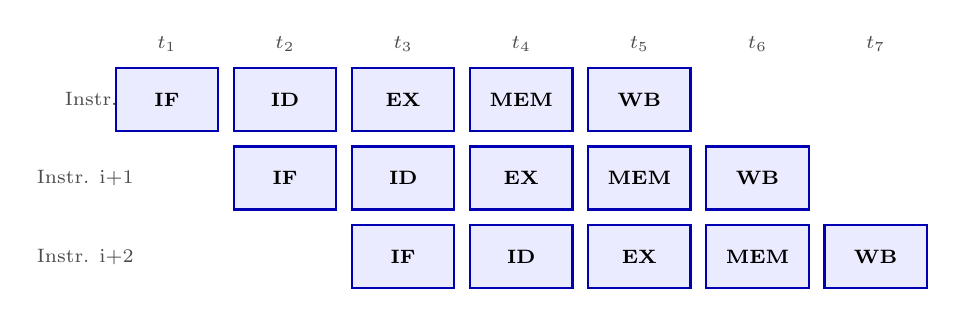
\begin{tikzpicture}[
    stage/.style={rectangle, draw=blue!70!black, fill=blue!8, thick, minimum width=1.3cm, minimum height=0.8cm, align=center, font=\scriptsize\bfseries},
    lbl/.style={font=\scriptsize, text=gray!60!black}
]
    \foreach \i/\name/\y in {0/i/0, 1/i+1/-1, 2/i+2/-2} {
        \node[lbl, anchor=east] at (-0.3, \y) {Instr. \name};
    }
    \foreach \s [count=\c from 0] in {IF,ID,EX,MEM,WB} {
        \node[stage] at (\c*1.5, 0) {\s};
    }
    \foreach \s [count=\c from 1] in {IF,ID,EX,MEM,WB} {
        \node[stage] at (\c*1.5, -1) {\s};
    }
    \foreach \s [count=\c from 2] in {IF,ID,EX,MEM,WB} {
        \node[stage] at (\c*1.5, -2) {\s};
    }
    \node[lbl] at (0, 0.7) {$t_1$};
    \foreach \t [count=\c from 2] in {2,...,7} {
        \node[lbl] at (\c*1.5-1.5, 0.7) {$t_{\c}$};
    }
\end{tikzpicture}
\caption{Overlap of the five pipeline stages across consecutive instructions.}
\label{fig:pipeline-5-stadi-en}
\end{figure}

\subsection{Latency, Throughput, and Pipeline Depth}

Let $k$ be the number of pipeline stages and $\tau$ the clock cycle period. The \textbf{latency} $L$ is the total time required for a single instruction to traverse the entire pipeline, $L = k \cdot \tau$: in modern CPUs the latency for a simple operation typically ranges between $10$ and $20$ clock cycles. The \textbf{throughput} $W$ is the number of instructions completed per unit time, and at steady state $W = 1/\tau$ instructions per second, since one instruction exits the pipeline every cycle. The period $\tau$ is dictated by the delay of the slowest stage in the circuit chain,
\[
\tau \ge \max_{1 \le i \le k} \left(t_{\text{stage}_i}\right).
\]
To raise the clock frequency (reduce $\tau$), designers increase pipeline depth $k$ (up to 15--20 or more stages in modern CPUs), implementing each stage with simpler, faster circuitry; conversely, increasing $k$ inflates the penalty in case of a forced pipeline flush.

\FloatBarrier
\section{Superscalar Execution, Interleaving, and Structural Hazards}

A processor is called \textbf{superscalar} when it has the architectural ability to issue and complete more than one instruction per clock cycle ($IPC > 1$, \textit{Instructions Per Cycle}) within the same core, integrating multiple arithmetic-logic units (integer ALUs, multipliers, shift units, load/store units) served by parallel issue ports (\textit{execution ports}). Real architectures such as Intel Haswell feature, for instance, a 56-entry decode queue, a 192-entry reorder buffer, a unified 60-entry reservation station, and 8 parallel execution ports, each specialized for classes of operations (integer ALUs, load/store, vector units, branch, etc.).

\subsection{The Arithmetic \textit{Interleaving} Experiment}

Four Rust functions operating on a vector of 64-bit integers \texttt{\&[u64]} are benchmarked, accumulating an increasing number of independent operations per iteration.

\begin{lstlisting}[style=rustcode,caption={From a single reduction to four independent reductions per iteration.}]
pub fn do_stuff(v: &[u64]) -> u64 {
    let mut prod = 1;
    for &value in v.iter() {
        prod *= value;
    }
    prod
}

pub fn do_more_stuff(v: &[u64]) -> (u64, u64) {
    let mut prod = 1;
    let mut sum = 0;
    for &value in v.iter() {
        prod *= value;
        sum += value;
    }
    (prod, sum)
}

pub fn do_more_stuff_2(v: &[u64]) -> (u64, u64, u64) {
    let mut prod = 1;
    let mut sum = 0;
    let mut xor = 0;
    for &value in v.iter() {
        prod *= value;
        sum += value;
        xor ^= value;
    }
    (prod, sum, xor)
}

#[inline]
pub fn do_more_stuff_3(v: &[u64]) -> (u64, u64, u64, u64) {
    let mut prod = 1;
    let mut sum = 0;
    let mut xor = 0;
    let mut or = 0;
    for &value in v.iter() {
        prod *= value;
        sum += value;
        xor ^= value;
        or |= value;
    }
    (prod, sum, xor, or)
}
\end{lstlisting}

\begin{table}[htbp]
\centering
\small
\begin{tabular}{l r}
\toprule
\textbf{Function} & \textbf{Time per iteration} \\
\midrule
\texttt{do\_stuff()} (1 operation) & $0.4\,\text{ns}$ \\
\texttt{do\_more\_stuff()} (2 operations) & $0.4\,\text{ns}$ \\
\texttt{do\_more\_stuff\_2()} (3 operations) & $0.4\,\text{ns}$ \\
\texttt{do\_more\_stuff\_3()} (4 operations) & $0.5\,\text{ns}$ \\
\bottomrule
\end{tabular}
\caption{Time per iteration as the number of accumulated independent reductions grows.}
\label{tab:interleaving-arithmetic-en}
\end{table}

\subsection{Instruction Overlap and Port Saturation}

From one to three operations the time remains unchanged at $0.4\,\text{ns}$ because the accumulator variables have no mutual dependencies: $\text{prod}_{t+1} = \text{prod}_t \cdot v[i]$, $\text{sum}_{t+1} = \text{sum}_t + v[i]$, $\text{xor}_{t+1} = \text{xor}_t \oplus v[i]$. The superscalar core simultaneously dispatches the multiplication, addition, and XOR to three distinct execution ports: the three operations complete in the same clock cycle, and the extra work is performed at zero cost.

With the fourth operation (\texttt{or}) the time rises to $0.5\,\text{ns}$ rather than doubling to $0.8\,\text{ns}$: this is a \textbf{structural hazard}, since the physical units available for parallel arithmetic-logic computation in a single cycle are saturated (only three instructions of that type can be issued simultaneously), and one of the four operations must wait. However the \textit{out-of-order} CPU does not process iterations as isolated compartments: it implicitly unrolls the instruction window, grouping them into blocks of three, absorbing the excess operation into subsequent cycles and saturating the residual capacity of the ports. The real overhead thus amounts to a marginal fraction of a cycle ($\Delta t = +0.1\,\text{ns}$) rather than a full additional cycle.

\FloatBarrier
\section{Data Hazards and Serial Dependencies}

\begin{definition}[Data Hazard]
A \textbf{data hazard} occurs when an instruction needs an operand that is not yet available because it is still being computed by a preceding instruction. It corresponds to a \textbf{RAW} (\textit{Read-After-Write}) data dependency:
\[
\text{Inst}_A:\ R_1 \leftarrow R_2 + R_3 \qquad \Longrightarrow \qquad \text{Inst}_B:\ R_4 \leftarrow R_1 \times R_5,
\]
where $\text{Inst}_B$ must stall in the pipeline until $\text{Inst}_A$ completes its computation.
\end{definition}

Consider code that performs the same number of operations per iteration as the previous \texttt{do\_more\_stuff\_3}, but chains the data in a tight dependency:

\begin{lstlisting}[style=rustcode,caption={Serial RAW dependency chain across four operations.}]
pub fn do_more_stuff_4(v: &[u64]) -> (u64, u64, u64) {
    let mut prod = 1;
    let mut sum = 0;
    let mut xor = 0;
    for &value in v.iter() {
        sum += value;  // 1. compute sum
        prod *= sum;   // 2. tightly depends on sum
        xor ^= prod;   // 3. tightly depends on prod
        sum += xor;    // 4. depends on xor and overwrites sum for the next iteration!
    }
    (prod, sum, xor)
}
\end{lstlisting}

Because of the RAW chain, the execution units cannot start any computation in parallel:
\[
\text{Iteration latency} = t_{\text{add}} + t_{\text{mul}} + t_{\text{xor}} + t_{\text{add\_feedback}}.
\]
Since the last operation updates \texttt{sum} and the first instruction of the next iteration requires the new value of \texttt{sum}, the \textit{out-of-order} CPU cannot start iteration $t+1$ early: the superscalar units remain unused. Experimentally, against the $0.5\,\text{ns}$ of \texttt{do\_more\_stuff\_3} (independent operations), \texttt{do\_more\_stuff\_4} measures $1.7\,\text{ns}$ per iteration ($\approx 3.5\times$ slower), despite performing the same number of arithmetic operations.

\subsection{Algorithmic Solution: \textit{Interleaving} Independent Vectors}

When the same function with a tight dependency must be run on two distinct vectors \texttt{V} and \texttt{West}, the traditional sequential approach (\texttt{do\_more\_stuff\_4(V)} followed by \texttt{do\_more\_stuff\_4(West)}) takes an overall time $2T$. If instead a single function processes both vectors within the same iteration, alternating the two independent chains:

\begin{lstlisting}[style=rustcode,caption={Fusion (interleaving) of two mutually independent RAW chains.}]
for i in 0..n {
    // chain for V (occupies the ports at cycle k)
    sum_v += v[i];
    prod_v *= sum_v;
    xor_v ^= prod_v;
    sum_v += xor_v;
    // chain for West, completely independent of V!
    sum_w += west[i];
    prod_w *= sum_w;
    xor_w ^= prod_w;
    sum_w += xor_w;
}
\end{lstlisting}

the measured execution time is identical to that of the single vector \texttt{V} alone ($\approx T$, rather than $2T$). Operations on \texttt{West} do not depend on those on \texttt{V}: while \texttt{V}'s chain is waiting for ALU results, the free compute units process \texttt{West}'s chain, filling the dead time imposed by data dependencies at zero extra cost.

\FloatBarrier
\section{Control Hazards, Speculative Execution, and Branch Prediction}

\begin{definition}[Control Hazard]
A \textbf{control hazard} occurs when the CPU cannot determine which instruction to fetch next (\textit{instruction fetch}) due to the presence of a conditional branch (\texttt{if}, \texttt{branch}).
\end{definition}

The CPU cannot stop at every condition: it therefore adopts \textbf{speculative execution}, guessing via a \textit{branch predictor} which branch will be taken and speculatively fetching subsequent instructions to feed the pipeline. If the outcome of the condition turns out to disagree with the prediction, all speculative work completed in the intermediate stages must be discarded, with a full pipeline flush and reload from the correct branch:
\[
\text{Misprediction penalty} = 15\text{--}20 \text{ clock cycles}.
\]

\subsection{The Random Condition Paradox}

A conditional filter is introduced into code with a dependency chain, operating on an array of random integers uniformly distributed in $[0, 99]$:

\begin{lstlisting}[style=rustcode,caption={Conditional branch on random values: the CPU cannot predict the outcome.}]
pub fn do_more_stuff_5(v: &[u64]) -> (u64, u64, u64) {
    let mut prod = 1;
    let mut sum = 0;
    let mut xor = 0;
    for &value in v.iter() {
        if value > 50 { // true with p = 0.5 on random values in [0, 99]
            sum += value;
            prod *= sum;
            xor ^= prod;
            sum += xor;
        }
    }
    (prod, sum, xor)
}
\end{lstlisting}

Since the condition is true on average $50\%$ of the time, one would intuitively expect a time roughly halved compared to \texttt{do\_more\_stuff\_4} ($1.7 / 2 \approx 0.85\,\text{ns}$). The measured time instead rises to $3.5\,\text{ns}$, more than twice as slow as the version without the condition.

\begin{alertblock}{The Real Cost Is Not Computation but Misprediction}
With random values the branch predictor's accuracy is equivalent to a coin flip, $P(\text{hit}) = P(\text{miss}) = 0.50$. The average cost per iteration is then
\[
\text{Average cost} \approx 0.5 \times T_{\text{body}} + P(\text{miss}) \times \text{Flush penalty}
\approx 0.5 \times 0.85\,\text{ns} + 0.5 \times 5.0\,\text{ns} \approx 2.9\text{--}3.5\,\text{ns},
\]
having assumed a penalty of $15$--$20$ cycles ($\approx 4$--$5\,\text{ns}$ on a $4\,\text{GHz}$ CPU). The cost of the algorithm is no longer dictated by arithmetic operations, but is dominated by the time lost flushing and refilling the pipeline.
\end{alertblock}

\subsection{Experimental Verification: Data Ordering and Periodic Patterns}

To demonstrate that the slowdown derives exclusively from branch predictor behavior, the same identical code is run while only changing the arrangement of data in the array.

\begin{table}[htbp]
\centering
\small
\begin{tabular}{l r l}
\toprule
\textbf{Configuration} & \textbf{Time per iteration} & \textbf{Predictor behavior} \\
\midrule
\texttt{do\_more\_stuff\_4()} (no \texttt{if}) & $1.7\,\text{ns}$ & --- \\
\texttt{do\_more\_stuff\_5()}, random data & $3.5\,\text{ns}$ & unpredictable branch, miss rate $\approx 50\%$ \\
\texttt{do\_more\_stuff\_5()}, sorted data & $1.2\,\text{ns}$ & near-perfect prediction, single miss \\
\texttt{do\_more\_stuff\_5()}, alternating data & $1.1\,\text{ns}$ & periodic sequence, miss rate $\approx 0\%$ \\
\bottomrule
\end{tabular}
\caption{Time per iteration of \texttt{do\_more\_stuff\_5()} as data arrangement varies.}
\label{tab:branch-prediction-benchmark-en}
\end{table}

With \textbf{sorted data} (all elements $\le 50$ at the start of the array and all elements $> 50$ at the end) the predictor assumes the branch is not taken for the whole first half and taken for the second: a single misprediction occurs at the transition point, and once flush costs are removed the time drops to $1.2\,\text{ns}$, lower than the $1.7\,\text{ns}$ of the version without the condition since half the iterations do not execute the \texttt{if} body. With \textbf{alternating data} following a periodic pattern (\textit{false, true, false, true, \ldots}), predictors integrate historical pattern tables (\textit{branch history shift register}): once the periodicity is identified, the predictor anticipates the outcome at every step without errors, eliminating stalls.

\subsection{\textit{Branchless} Techniques and the Implicit Jump of \texttt{for} Loops}

If data cannot be sorted or predicted, the only solution is to physically remove the conditional branch (\textit{branchless code}), replacing it with algebraic expressions or conditional assembly instructions (\texttt{CMOV}). For example, instead of
\begin{lstlisting}[style=rustcode]
if value > 50 {
    sum += value;
}
\end{lstlisting}
the logical guard is mapped onto a scalar binary value ($0$ or $1$), always performing the arithmetic operation:
\begin{lstlisting}[style=rustcode]
let condition = (value > 50) as u64; // 1 if true, 0 if false
sum += value * condition;            // adds 'value' if true, adds '0' if false
\end{lstlisting}
The program always performs the mathematical computation, but the instruction flow is linear: there are no branches, and mispredictions are eliminated.

\begin{remark}[Why the \texttt{for} Loop Branch Is Not a Problem]
Every \texttt{for} loop ends at the machine level with a conditional jump back to the start of the block. This branch does not degrade performance because it is highly asymmetric: for $N$ iterations, the loop-continuation condition is true $N-1$ consecutive times and false only upon exit. The branch predictor immediately learns the pattern (``branch taken'') and commits a single misprediction at the end of the loop, with a completely negligible impact on overall time.
\end{remark}

\FloatBarrier
\section{Synthesis: From Hardware Constraints to Algorithmic Choices}

The phenomena analyzed in this chapter -- memory hierarchy and locality, pipelining, superscalar execution, \textit{data hazards}, and \textit{control hazards} -- are not negligible implementation details, but physical constraints that determine the actual performance behavior of large-scale Information Retrieval algorithms. In particular:

\begin{itemize}
    \item data structures (posting lists, inverted indexes) should be designed to favor sequential, contiguous access, in order to exploit spatial locality and hardware prefetching;
    \item when possible, it is beneficial to express multiple independent reductions within the same loop to saturate superscalar execution ports at marginal cost;
    \item tight (RAW) dependency chains between accumulator variables should be identified and, where possible, decoupled or interleaved with independent computations from other data streams;
    \item unpredictable conditional branches on data-dependent conditions should be replaced with branchless techniques whenever the misprediction cost outweighs the extra computation.
\end{itemize}
